
\documentclass[11pt,letterpaper]{article}

% Load some basic packages that are useful to have
% and that should be part of any LaTeX installation.
%
% be able to include figures
\usepackage{graphicx}
% get nice colors
\usepackage{xcolor}

% change default font to Palatino (looks nicer!)
\usepackage[latin1]{inputenc}
\usepackage{mathpazo}
\usepackage[T1]{fontenc}
% load some useful math symbols/fonts
\usepackage{latexsym,amsfonts,amsmath,amssymb}

% comfort package to easily set margins
\usepackage[top=1in, bottom=1in, left=1in, right=1in]{geometry}
\usepackage{hyperref}
\usepackage[all]{hypcap}
% control some spacings
%
% spacing after a paragraph\begin{figure}[bth]
\setlength{\parskip}{.15cm}
% indentation at the top of a new paragraph
\setlength{\parindent}{0.0cm}

\begin{document}

\begin{center}
\Large
Ay190 -- Worksheet 10\\
David Vartanyan\\
Date: \today
\end{center}

\section{}

We use the shooting method code template to solve our BVP. We guess a $z=y'(a)$ and use an integrator (FE or RK2) to extend to boundary $b$. We calculate the error between $y(z)$ and our endpoint $B=y(b)$. We then use a rootfinder to improve our guess of $z$ and iterate until desired accuracy. Even with extreme values of $z$, the process takes 2 iterations (see ws10.py and ws10b.py).

To test for convergence, we run using $10$ and $10000$ steps. FE converges, see ~\ref{fig:1} and ~\ref{fig:2}; interestingly, RK2 doesn't. See ~\ref{fig:3} and ~\ref{fig:4}.

The top figure shows the exact and FE or RK2 solution to our BVP; the subplot shows the error. RK2 is accurate but divergent.

\begin{figure}[bth]
\centering
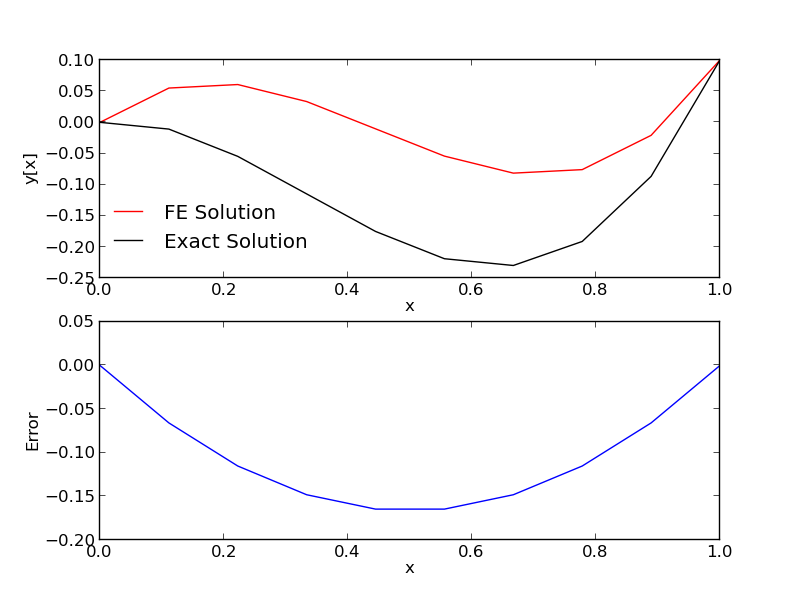
\includegraphics[width=0.7\textwidth]{ws101a.png}
\caption{FE, npoints=10}
\label{fig:1}
\end{figure}

\begin{figure}[bth]
\centering
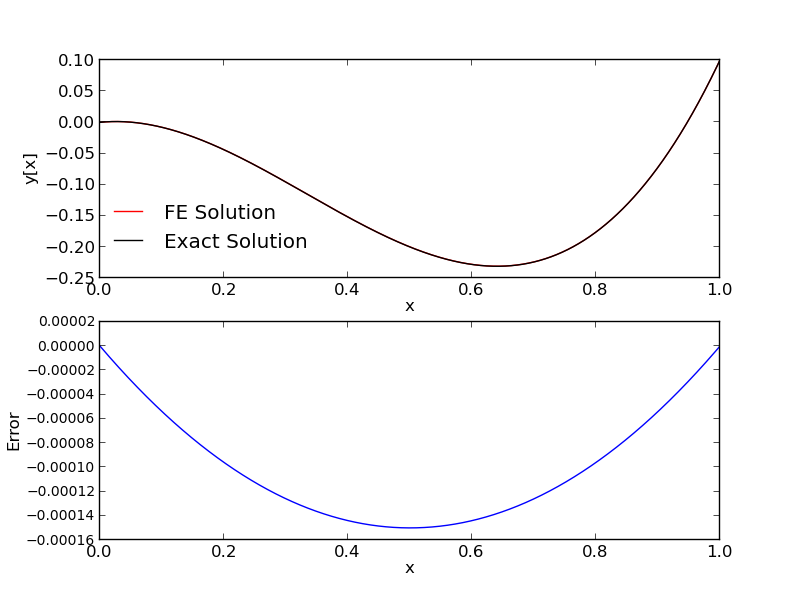
\includegraphics[width=0.7\textwidth]{ws101b.png}
\caption{FE, npoints=10000}
\label{fig:2}
\end{figure}

\begin{figure}[bth]
\centering
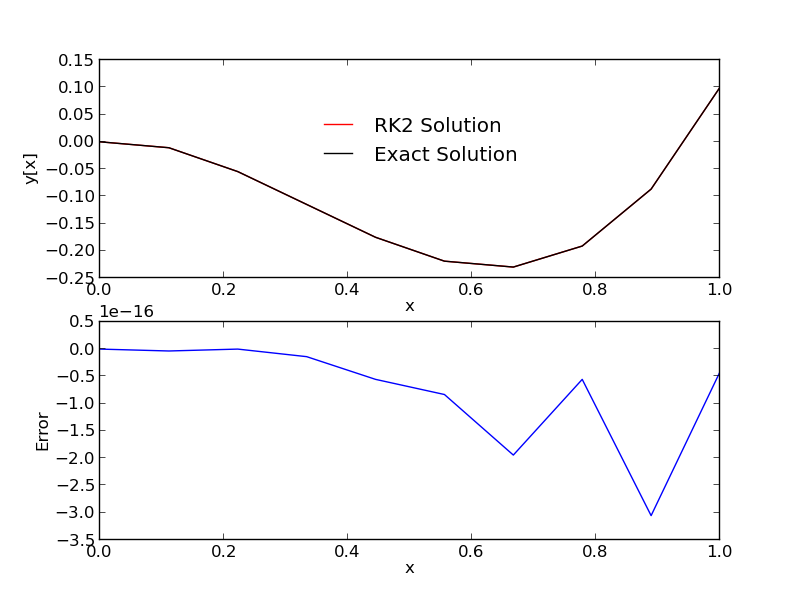
\includegraphics[width=0.7\textwidth]{ws102a.png}
\caption{RK2, npoints=10}
\label{fig:3}
\end{figure}

\begin{figure}[bth]
\centering
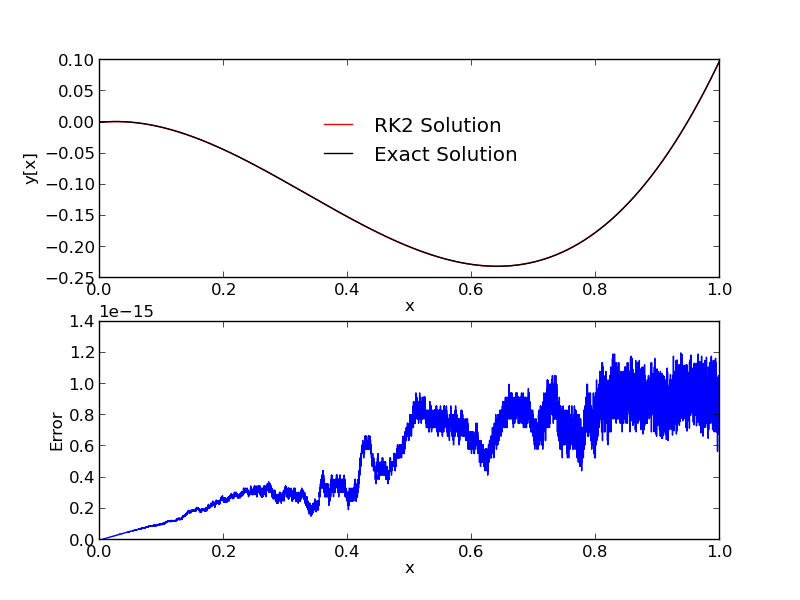
\includegraphics[width=0.7\textwidth]{ws102b.png}
\caption{RK2, npoints=10000}
\label{fig:4}
\end{figure}

\end{document}
